
Metal/oxide interfaces are among most important heterogeneous structures because various thin films are present in optical coatings, semiconductor devices and catalysts. Therefore it is important to understand the thin film stability and morphology evolution during deposition processes. From this study, we will understand: (1) What are the major factors that affect metal thin film morphology during deposition? (2) How do we improve the wettability of metallic thin films on the oxide substrates?

To answer these two questions, \ac{GCMC} simulations are conducted on various substrate based on Ag-substrate bonding strength obtained from H-saturated ZnO (000$\overline{1}$) surfaces, with different lattice constants and substrate orientations. Among these parameters, substrate orientation is critical to Ag thin film quality. It turns out that the hexagonal substrate is robust for Ag thin film growth under different lattice constants and yields best Ag thin film quality with (111) orientation, because misfit dislocations are easier to generate hence helping interface stress released. 
%Besides, several polycrstalline substrate cases are also studied to consider more realistic case.
By adding trace amount of ``anchor'' sites on the substrate, thin film morphology becomes much smoother and more continuous. Then high throughput \ac{DFT} calculations are used to identify potential ``anchor'' elements. Five elements, Pd, Sb, Se, Sn and Te, are found to have the ability to act as ``anchor'' site elements that can increase Ag nucleation densities on substrates that have weak bonding to metallic thin films.

\section{Introduction}

Low-emission glasses are used for architectures widely. It is used to achieve better energy efficiency by minimizing the ultraviolet and infrared light that can pass through while not significantly compromising the amount of visible light. Multi-layer structures, as shown in Figure \ref{Chap:Ag/ZnO:fig:1a}, are used for this purpose. Most of the multi-layer structures are repeating ``dielectric layer/low-emission layer/dielectric layer'' units.

Typical low-emission layers can be noble metals, e.g. Ag. The ability of a material to radiate energy is known as emissivity. In general, highly reflective materials, such as silver or aluminum, have a low emissivity. For example, untreated glass has an emissivity of 0.84, while silver has an emissivity of under 0.06. \cite{salisbury1992emissivity} Hence, reducing the emissivity of the window glass by coating Ag can improve the insulating property of architectural glasses. Dielectric layers are necessary to form an inferential filter that grants the reflection of the visible wavelengths to be reduced and consequently increases the light transmission. Another reason to utilize dielectric layers is that the reflected fraction in the visible results in as neutral a color as possible, and in particular so that the reflection does not lead to purple stains which are against human preferences. Moreover, the choice of dielectric layers or systems of dielectric layers is such that neutrality in reflection is realized for the broadest range of angles of incidence to the glazing. And oxides, e.g. ZnO, are usually great dielectric materials.

\newpage
\begingroup
\begin{figure}[!ht]
  \centering
  \subfigure{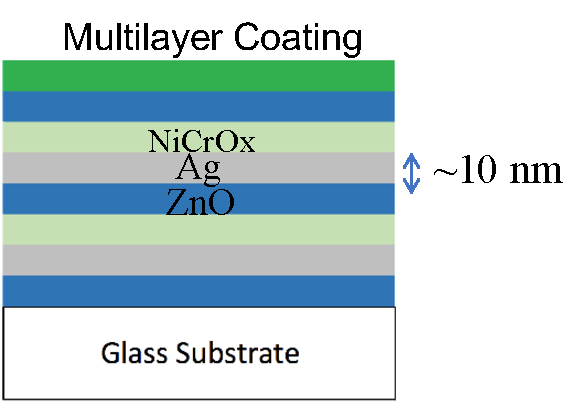
\includegraphics[width=0.75\linewidth]{Chap4/plots/Picture1a.pdf}}\label{Chap:Ag/ZnO:fig:1a}
\caption[Illustration of multi-layer structures and thin film morphology]{Illustration of multi-layer structures of architecture glass.}
  \label{Chap:Ag/ZnO:fig1}
\end{figure}
\endgroup

However, Ag/ZnO interface has weaker adhesion energy compared to many other metal/oxide interfaces. The strengths of adhesion between metals and oxides can largely affect the wetting behaviors and morphology of interfaces. On the other hand, defects, like islands forming, high surface roughness and high density of pinholes, will all reduce the satisfactory of glass quality, as shown in Liu's paper \cite{liu2013lithography}. For industrial practices, Ag thin film deposited on ZnO layers is usually above 10 nm thickness so as to guarantee continuous thin film. Therefore, to achieve continuous thin film with thinner layers can improve the cost efficiency by reducing the amount of Ag needed.

In this chapter, attention was paid to mainly two parts: 1) the effect of substrate on the Ag thin film quality; 2) the effect of alloy segregation at Ag grain boundary on the Ag thin film stability. \ac{GCMC} methods will be used to study the morphology of Ag thin film on different substrates with various substrate structures, lattice constant and bonding strength to Ag atoms. The goal of this study is to simulate the morphology after annealing, hence detailed kinetics, like bombardment effects, can be ignored. Therefore, \ac{GCMC} simulation will be a suitable tool, because it is based on the thermodynamic driving force. On the other hand, \ac{DFT} calculations will be used to study the segregation of alloy elements at different Ag grain boundaries.


\section{Conclusions}
In this chapter, we studied how does substrate affect Ag thin film morphology by using \ac{GCMC} and empirical potentials. This method is expandable to other metal thin films as well as other substrates, like MgO.

We found that only Ag films on the hexagonal substrate are robust to substrate lattice constant and bonding strength changes, and yields most \{111\} orientation Ag. Therefore, Ag thin film quality (improve texture and reduce internal defects) can be improved by increasing ZnO substrate quality. 

In order to achieve more continuous Ag thin films with less Ag, some elements can be added as ``anchor'' sites to incoming Ag atoms. Pd, Sb, Se, Sn, and Te can be good candidates as ``anchor'' sites on the ZnO substrate. With trace amount (0.05\ac{ML}) of ``anchor'' sites on the substrate, more nuclei can be achieved, hence more continuous ultra-thin film.

We also tried to search doping elements that can segregate in Ag grain boundaries to stabilize grain size during heat treatments. First-principles calculation showed transition metals, e.g. W, do not segregation in Ag grain boundaries, which is inconsistent with experiments. We suspect that alloying elements can not only change chemistry of the grain boundaries, but also disrupt the atomistic structure of grain boundaries in alloys. Therefore, an evolutionary algorithm to search stable complex grain boundaries for binary alloy need to be used. Besides, the electronic mechanism also needs to be investigated.